% ============================================================
% Figure 4: OPD Failure Progression (3-panel, full width)
% ============================================================
\begin{figure*}[t]
\centering
\begin{subfigure}[b]{0.33\textwidth}
\centering
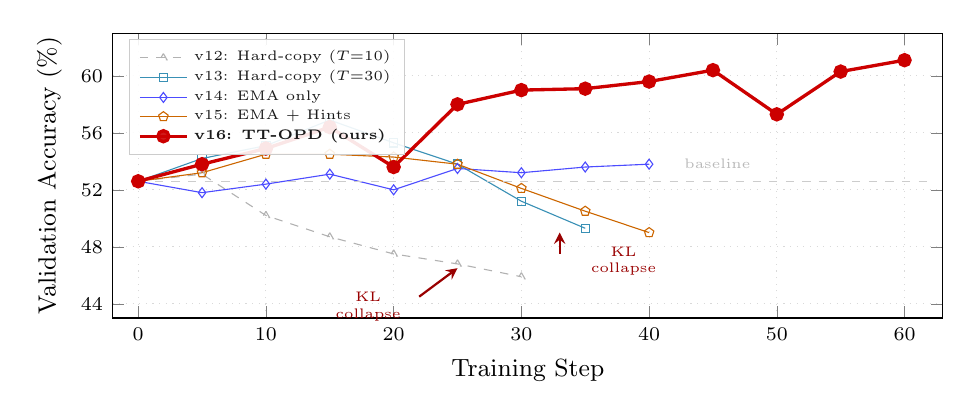
\begin{tikzpicture}
\begin{axis}[
    width=\textwidth,
    height=5.2cm,
    xlabel={Training Step},
    ylabel={Validation Accuracy (\%)},
    xmin=-2, xmax=63,
    ymin=43, ymax=63,
    xtick={0,10,20,30,40,50,60},
    ytick={44,48,52,56,60},
    grid=major,
    grid style={dotted, gray!30},
    tick label style={font=\scriptsize},
    label style={font=\small},
    legend style={at={(0.02,0.98)}, anchor=north west, font=\fontsize{5.5}{6.5}\selectfont, row sep=-2pt, draw=gray!40, fill=white, fill opacity=0.9},
    legend cell align={left},
    clip=false,
]
% v12 (Hard-copy T=10) -- dashed, thin
\addplot[color=gray!60, mark=triangle, mark size=1.5pt, thin, dashed] coordinates {
    (0,52.6) (5,53.1) (10,50.2) (15,48.7) (20,47.5) (25,46.8) (30,45.9)
};
\addlegendentry{v12: Hard-copy ($T{=}10$)}

% v13 (Hard-copy T=30) -- thin
\addplot[color=cyan!70!black, mark=square, mark size=1.5pt, thin] coordinates {
    (0,52.6) (5,54.2) (10,55.1) (15,56.9) (20,55.3) (25,53.8) (30,51.2) (35,49.3)
};
\addlegendentry{v13: Hard-copy ($T{=}30$)}

% v14 (EMA only) -- thin
\addplot[color=blue!70, mark=diamond, mark size=1.8pt, thin] coordinates {
    (0,52.6) (5,51.8) (10,52.4) (15,53.1) (20,52.0) (25,53.5) (30,53.2) (35,53.6) (40,53.8)
};
\addlegendentry{v14: EMA only}

% v15 (EMA+Hints) -- thin
\addplot[color=orange!80!black, mark=pentagon, mark size=1.8pt, thin] coordinates {
    (0,52.6) (5,53.2) (10,54.5) (15,54.5) (20,54.3) (25,53.8) (30,52.1) (35,50.5) (40,49.0)
};
\addlegendentry{v15: EMA + Hints}

% v16 (Full TT-OPD) -- BOLD RED
\addplot[color=red!80!black, mark=*, mark size=2pt, very thick] coordinates {
    (0,52.6) (5,53.8) (10,54.9) (15,56.4) (20,53.6) (25,58.0) (30,59.0) (35,59.1) (40,59.6) (45,60.4) (50,57.3) (55,60.3) (60,61.1)
};
\addlegendentry{\textbf{v16: TT-OPD (ours)}}

% Baseline reference
\addplot[dashed, gray!40, very thin] coordinates {(0,52.6) (62,52.6)};
\node[font=\fontsize{5}{6}\selectfont, gray!55, anchor=south west] at (axis cs:42,52.8) {baseline};

% KL collapse arrow on v12
\draw[->, >=stealth, red!60!black, thick] (axis cs:22,44.5) -- (axis cs:25,46.5);
\node[font=\fontsize{5}{6}\selectfont, red!60!black, align=center] at (axis cs:18,43.8) {KL\\collapse};

% KL collapse arrow on v13
\draw[->, >=stealth, red!60!black, thick] (axis cs:33,47.5) -- (axis cs:33,49.0);
\node[font=\fontsize{5}{6}\selectfont, red!60!black, align=center] at (axis cs:38,47.0) {KL\\collapse};

\end{axis}
\end{tikzpicture}
\caption{Validation Accuracy}
\label{fig:opd_acc}
\end{subfigure}%
\hfill
\begin{subfigure}[b]{0.33\textwidth}
\centering
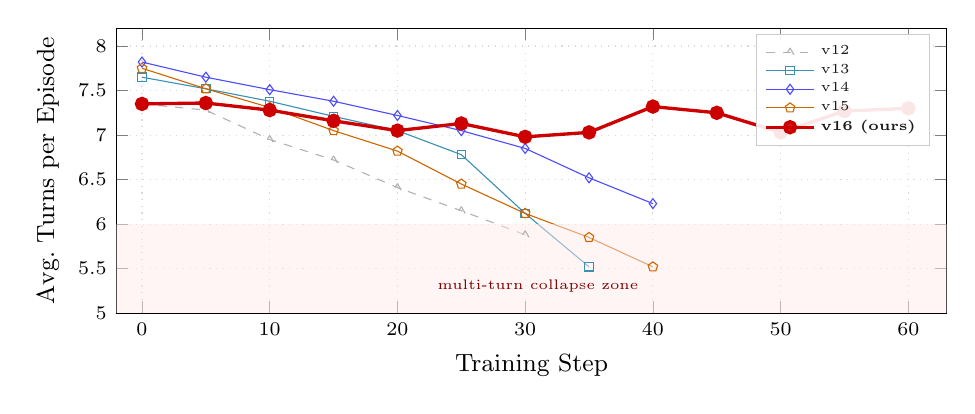
\begin{tikzpicture}
\begin{axis}[
    width=\textwidth,
    height=5.2cm,
    xlabel={Training Step},
    ylabel={Avg.\ Turns per Episode},
    xmin=-2, xmax=63,
    ymin=5.0, ymax=8.2,
    xtick={0,10,20,30,40,50,60},
    ytick={5.0,5.5,6.0,6.5,7.0,7.5,8.0},
    grid=major,
    grid style={dotted, gray!30},
    tick label style={font=\scriptsize},
    label style={font=\small},
    legend style={at={(0.98,0.98)}, anchor=north east, font=\fontsize{5.5}{6.5}\selectfont, row sep=-2pt, draw=gray!40, fill=white, fill opacity=0.9},
    legend cell align={left},
]
% v12
\addplot[color=gray!60, mark=triangle, mark size=1.5pt, thin, dashed] coordinates {
    (0,7.35) (5,7.28) (10,6.95) (15,6.72) (20,6.41) (25,6.15) (30,5.88)
};
\addlegendentry{v12}

% v13
\addplot[color=cyan!70!black, mark=square, mark size=1.5pt, thin] coordinates {
    (0,7.65) (5,7.52) (10,7.38) (15,7.21) (20,7.05) (25,6.78) (30,6.12) (35,5.52)
};
\addlegendentry{v13}

% v14
\addplot[color=blue!70, mark=diamond, mark size=1.8pt, thin] coordinates {
    (0,7.82) (5,7.65) (10,7.51) (15,7.38) (20,7.22) (25,7.05) (30,6.85) (35,6.52) (40,6.23)
};
\addlegendentry{v14}

% v15
\addplot[color=orange!80!black, mark=pentagon, mark size=1.8pt, thin] coordinates {
    (0,7.75) (5,7.52) (10,7.31) (15,7.05) (20,6.82) (25,6.45) (30,6.12) (35,5.85) (40,5.52)
};
\addlegendentry{v15}

% v16 -- BOLD RED
\addplot[color=red!80!black, mark=*, mark size=2pt, very thick] coordinates {
    (0,7.35) (5,7.36) (10,7.28) (15,7.16) (20,7.05) (25,7.13) (30,6.98) (35,7.03) (40,7.32) (45,7.25) (50,7.03) (55,7.27) (60,7.30)
};
\addlegendentry{\textbf{v16 (ours)}}

% Multi-turn collapse zone
\fill[red!8, opacity=0.5] (axis cs:-2,5.0) rectangle (axis cs:63,6.0);
\node[font=\fontsize{5}{6}\selectfont, red!50!black] at (axis cs:31,5.3) {multi-turn collapse zone};

\end{axis}
\end{tikzpicture}
\caption{Average Turns}
\label{fig:opd_turns}
\end{subfigure}%
\hfill
\begin{subfigure}[b]{0.33\textwidth}
\centering
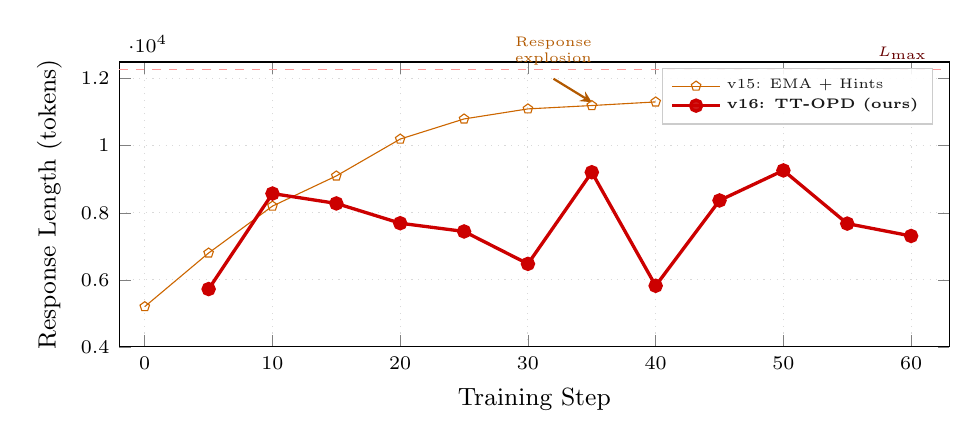
\begin{tikzpicture}
\begin{axis}[
    width=\textwidth,
    height=5.2cm,
    xlabel={Training Step},
    ylabel={Response Length (tokens)},
    xmin=-2, xmax=63,
    ymin=4000, ymax=12500,
    xtick={0,10,20,30,40,50,60},
    ytick={4000,6000,8000,10000,12000},
    yticklabel style={/pgf/number format/fixed, /pgf/number format/1000 sep={\,}},
    grid=major,
    grid style={dotted, gray!30},
    tick label style={font=\scriptsize},
    label style={font=\small},
    legend style={at={(0.98,0.98)}, anchor=north east, font=\fontsize{5.5}{6.5}\selectfont, row sep=-2pt, draw=gray!40, fill=white, fill opacity=0.9},
    legend cell align={left},
    clip=false,
]
% v15 response length -- shows explosion
\addplot[color=orange!80!black, mark=pentagon, mark size=1.8pt, thin] coordinates {
    (0,5200) (5,6800) (10,8200) (15,9100) (20,10200) (25,10800) (30,11100) (35,11200) (40,11308)
};
\addlegendentry{v15: EMA + Hints}

% v16 response length -- controlled
\addplot[color=red!80!black, mark=*, mark size=2pt, very thick] coordinates {
    (5,5724) (10,8574) (15,8279) (20,7689) (25,7443) (30,6476) (35,9210) (40,5822) (45,8368) (50,9264) (55,7677) (60,7308)
};
\addlegendentry{\textbf{v16: TT-OPD (ours)}}

% L_max line
\addplot[dashed, red!40, very thin] coordinates {(-2,12288) (63,12288)};
\node[font=\fontsize{5}{6}\selectfont, red!40!black, anchor=south east] at (axis cs:62,12288) {$L_{\max}$};

% Response explosion arrow on v15
\draw[->, >=stealth, orange!70!black, thick] (axis cs:32,12000) -- (axis cs:35,11300);
\node[font=\fontsize{5}{6}\selectfont, orange!70!black, align=center, anchor=south] at (axis cs:32,12100) {Response\\explosion};

\end{axis}
\end{tikzpicture}
\caption{Response Length}
\label{fig:opd_resplen}
\end{subfigure}
\caption{OPD failure progression across ablation variants. (a)~Validation accuracy: hard-copy variants (v12, v13) suffer KL collapse as the teacher becomes stale; EMA-only (v14) plateaus without outcome-aware signal; EMA+Hints (v15) initially improves but collapses without length control. Only TT-OPD (v16, bold red) achieves sustained improvement to 61.1\%. (b)~Average turns: v12--v15 exhibit monotonic decline toward single-turn collapse ($<$6 turns); v16 maintains 7.0--7.4 turns throughout training. (c)~Response length: v15 shows unchecked response explosion toward $L_{\max}$; v16's cosine reward keeps responses bounded (5.7--9.3K tokens).}
\label{fig:opd_failure}
\end{figure*}


% ============================================================
% Figure 5: Gradient Signal Dilution
% ============================================================
\begin{figure}[t]
\centering
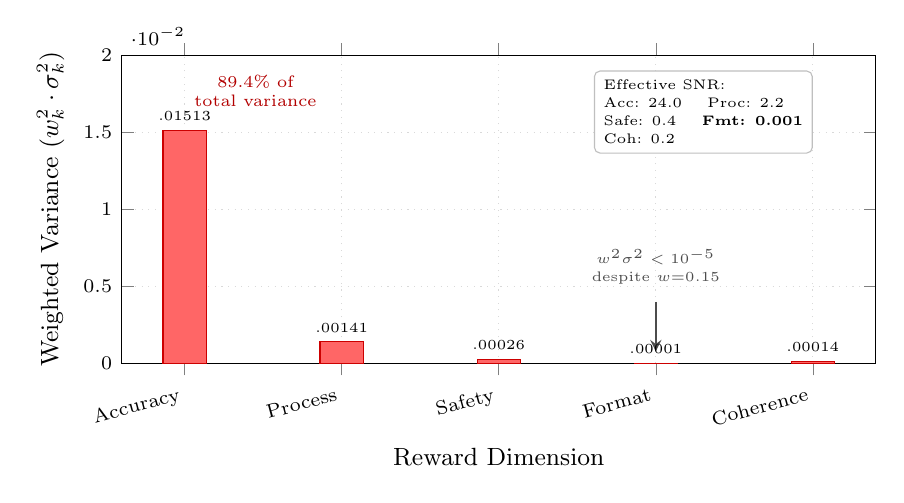
\begin{tikzpicture}
\begin{axis}[
    width=0.92\columnwidth,
    height=5.5cm,
    ybar,
    bar width=0.55cm,
    xlabel={Reward Dimension},
    ylabel={Weighted Variance ($w_k^2 \cdot \sigma_k^2$)},
    symbolic x coords={Accuracy, Process, Safety, Format, Coherence},
    xtick=data,
    xticklabel style={font=\scriptsize, rotate=15, anchor=north east},
    ymin=0, ymax=0.020,
    ytick={0, 0.005, 0.010, 0.015, 0.020},
    grid=major,
    grid style={dotted, gray!30},
    tick label style={font=\scriptsize},
    label style={font=\small},
    nodes near coords,
    every node near coord/.append style={font=\fontsize{5.5}{6.5}\selectfont, anchor=south},
    point meta=explicit symbolic,
    clip=false,
]
% w_k^2 * sigma_k^2:
% Accuracy: 0.30^2 * 0.41^2 = 0.09 * 0.1681 = 0.015129
% Process:  0.25^2 * 0.15^2 = 0.0625 * 0.0225 = 0.001406
% Safety:   0.20^2 * 0.08^2 = 0.04 * 0.0064 = 0.000256
% Format:   0.15^2 * 0.02^2 = 0.0225 * 0.0004 = 0.000009
% Coherence:0.10^2 * 0.12^2 = 0.01 * 0.0144 = 0.000144
\addplot[fill=red!60!white, draw=red!80!black] coordinates {
    (Accuracy, 0.01513) [.01513]
    (Process, 0.00141) [.00141]
    (Safety, 0.00026) [.00026]
    (Format, 0.00001) [.00001]
    (Coherence, 0.00014) [.00014]
};

% Annotation: Format negligible
\draw[->, >=stealth, gray!60!black, thick] (axis cs:Format, 0.004) -- (axis cs:Format, 0.0008);
\node[font=\fontsize{5.5}{6.5}\selectfont, gray!60!black, align=center, anchor=south] at (axis cs:Format, 0.0045) {$w^2\sigma^2 < 10^{-5}$\\despite $w{=}0.15$};

% Annotation: Accuracy dominates
\node[font=\fontsize{6}{7}\selectfont, red!70!black, align=center, anchor=south west] at (axis cs:Accuracy, 0.016) {89.4\% of\\total variance};

% Effective SNR box
\node[draw=gray!50, fill=white, rounded corners=2pt, font=\fontsize{5.5}{6.5}\selectfont, align=left, anchor=north east] at (axis cs:Coherence, 0.019) {
    Effective SNR:\\
    Acc: 24.0 \quad Proc: 2.2\\
    Safe: 0.4 \quad \textbf{Fmt: 0.001}\\
    Coh: 0.2
};

\end{axis}
\end{tikzpicture}
\caption{Gradient signal dilution in the 5D reward. Weighted variance contribution ($w_k^2 \cdot \sigma_k^2$) per reward dimension at step 20 (24 rollouts). Accuracy dominates 89.4\% of the total advantage variance, while Format---despite carrying 15\% weight---contributes $<$0.001\% due to near-zero variance ($\sigma{=}0.02$). This 24:1 SNR ratio between accuracy and format explains the agentic-textual transfer gap: format compliance is effectively invisible to the gradient signal.}
\label{fig:gradient_dilution}
\end{figure}


% ============================================================
% Figure 6: Training Dynamics Dashboard (v16, 4-panel)
% ============================================================
\begin{figure*}[t]
\centering
\begin{subfigure}[b]{0.24\textwidth}
\centering
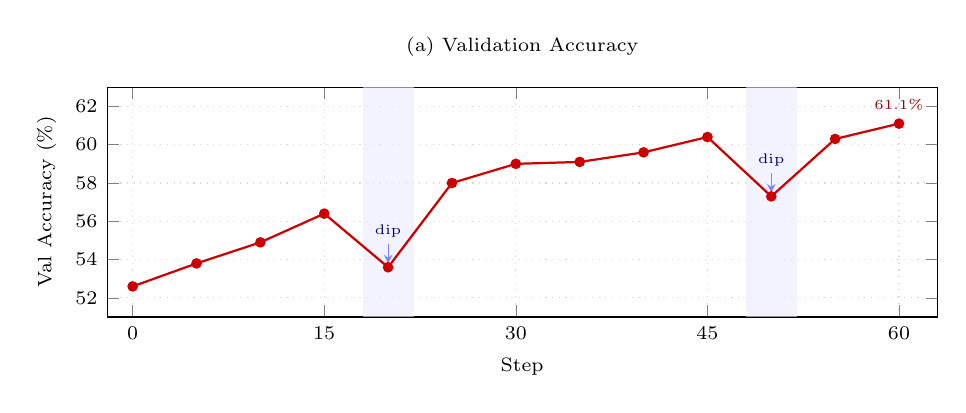
\begin{tikzpicture}
\begin{axis}[
    width=\textwidth,
    height=4.5cm,
    xlabel={Step},
    ylabel={Val Accuracy (\%)},
    xmin=-2, xmax=63,
    ymin=51, ymax=63,
    xtick={0,15,30,45,60},
    ytick={52,54,56,58,60,62},
    grid=major,
    grid style={dotted, gray!30},
    tick label style={font=\scriptsize},
    label style={font=\scriptsize},
    title={\scriptsize (a) Validation Accuracy},
    title style={at={(0.5,1.02)}},
]
% Shade dip regions
\fill[blue!8, opacity=0.6] (axis cs:18,51) rectangle (axis cs:22,63);
\fill[blue!8, opacity=0.6] (axis cs:48,51) rectangle (axis cs:52,63);

% v16 accuracy
\addplot[color=red!80!black, mark=*, mark size=1.5pt, thick] coordinates {
    (0,52.6) (5,53.8) (10,54.9) (15,56.4) (20,53.6) (25,58.0) (30,59.0) (35,59.1) (40,59.6) (45,60.4) (50,57.3) (55,60.3) (60,61.1)
};

% Oscillation annotations
\draw[->, >=stealth, blue!50, thin] (axis cs:20,54.8) -- (axis cs:20,53.8);
\node[font=\fontsize{4.5}{5.5}\selectfont, blue!50!black] at (axis cs:20,55.5) {dip};
\draw[->, >=stealth, blue!50, thin] (axis cs:50,58.5) -- (axis cs:50,57.5);
\node[font=\fontsize{4.5}{5.5}\selectfont, blue!50!black] at (axis cs:50,59.2) {dip};

% Peak arrows
\node[font=\fontsize{4.5}{5.5}\selectfont, red!60!black, anchor=south] at (axis cs:60,61.3) {61.1\%};

\end{axis}
\end{tikzpicture}
\end{subfigure}%
\hfill
\begin{subfigure}[b]{0.24\textwidth}
\centering
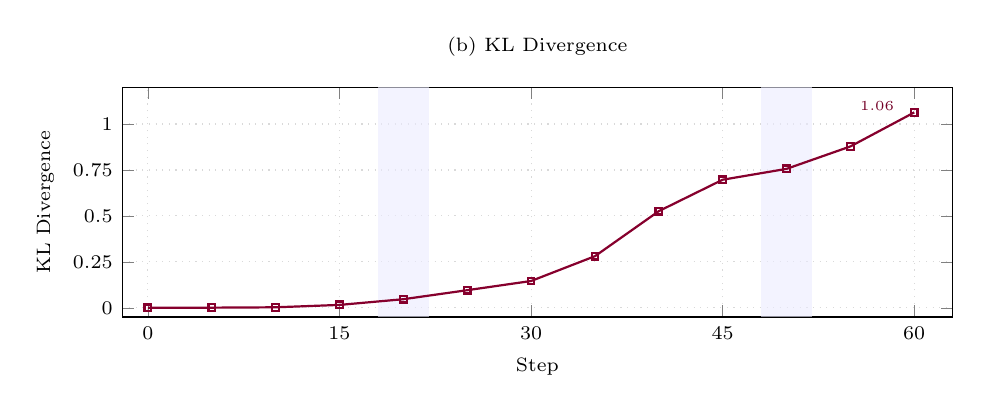
\begin{tikzpicture}
\begin{axis}[
    width=\textwidth,
    height=4.5cm,
    xlabel={Step},
    ylabel={KL Divergence},
    xmin=-2, xmax=63,
    ymin=-0.05, ymax=1.2,
    xtick={0,15,30,45,60},
    ytick={0, 0.25, 0.5, 0.75, 1.0},
    grid=major,
    grid style={dotted, gray!30},
    tick label style={font=\scriptsize},
    label style={font=\scriptsize},
    title={\scriptsize (b) KL Divergence},
    title style={at={(0.5,1.02)}},
]
% Shade dip regions
\fill[blue!8, opacity=0.6] (axis cs:18,-0.05) rectangle (axis cs:22,1.2);
\fill[blue!8, opacity=0.6] (axis cs:48,-0.05) rectangle (axis cs:52,1.2);

\addplot[color=purple!70!black, mark=square, mark size=1.2pt, thick] coordinates {
    (0,0) (5,0.001) (10,0.003) (15,0.016) (20,0.047) (25,0.096) (30,0.146) (35,0.281) (40,0.526) (45,0.697) (50,0.756) (55,0.878) (60,1.063)
};

\node[font=\fontsize{4.5}{5.5}\selectfont, purple!60!black, anchor=west] at (axis cs:55,1.1) {1.06};

\end{axis}
\end{tikzpicture}
\end{subfigure}%
\hfill
\begin{subfigure}[b]{0.24\textwidth}
\centering
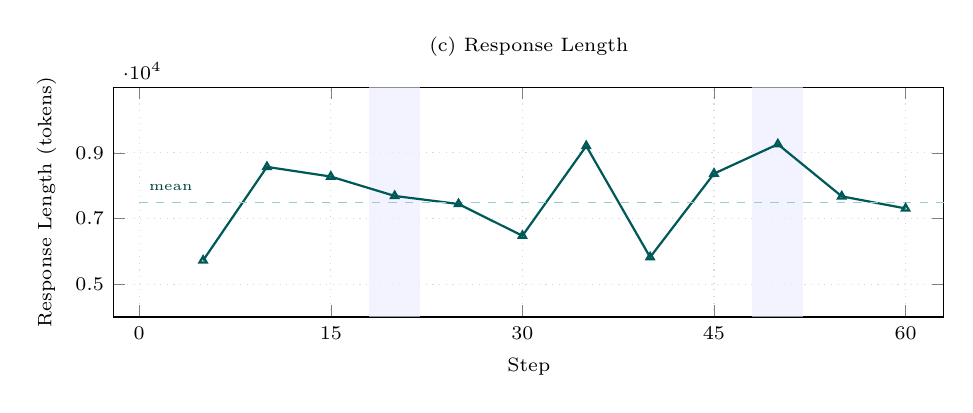
\begin{tikzpicture}
\begin{axis}[
    width=\textwidth,
    height=4.5cm,
    xlabel={Step},
    ylabel={Response Length (tokens)},
    xmin=-2, xmax=63,
    ymin=4000, ymax=11000,
    xtick={0,15,30,45,60},
    ytick={5000,7000,9000},
    yticklabel style={/pgf/number format/fixed, /pgf/number format/1000 sep={\,}},
    grid=major,
    grid style={dotted, gray!30},
    tick label style={font=\scriptsize},
    label style={font=\scriptsize},
    title={\scriptsize (c) Response Length},
    title style={at={(0.5,1.02)}},
]
% Shade dip regions
\fill[blue!8, opacity=0.6] (axis cs:18,4000) rectangle (axis cs:22,11000);
\fill[blue!8, opacity=0.6] (axis cs:48,4000) rectangle (axis cs:52,11000);

\addplot[color=teal!70!black, mark=triangle, mark size=1.5pt, thick] coordinates {
    (5,5724) (10,8574) (15,8279) (20,7689) (25,7443) (30,6476) (35,9210) (40,5822) (45,8368) (50,9264) (55,7677) (60,7308)
};

% Mean line
\addplot[dashed, teal!40, thin] coordinates {(0,7500) (63,7500)};
\node[font=\fontsize{4.5}{5.5}\selectfont, teal!50!black, anchor=south west] at (axis cs:0,7550) {mean};

\end{axis}
\end{tikzpicture}
\end{subfigure}%
\hfill
\begin{subfigure}[b]{0.24\textwidth}
\centering
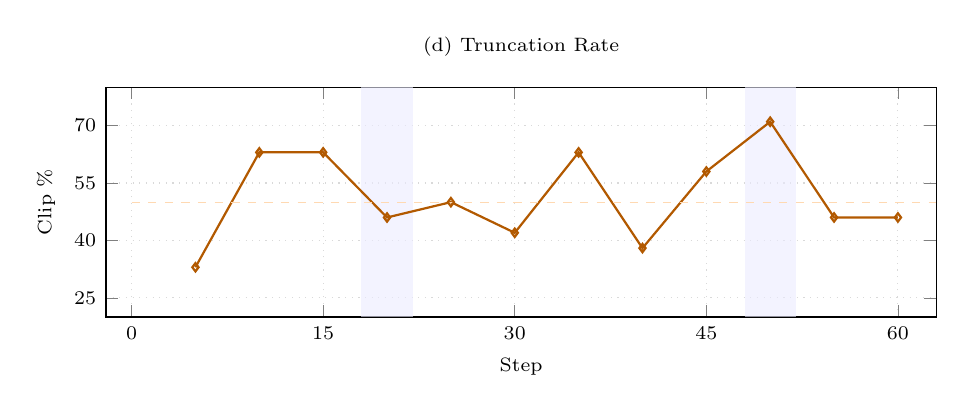
\begin{tikzpicture}
\begin{axis}[
    width=\textwidth,
    height=4.5cm,
    xlabel={Step},
    ylabel={Clip \%},
    xmin=-2, xmax=63,
    ymin=20, ymax=80,
    xtick={0,15,30,45,60},
    ytick={25,40,55,70},
    grid=major,
    grid style={dotted, gray!30},
    tick label style={font=\scriptsize},
    label style={font=\scriptsize},
    title={\scriptsize (d) Truncation Rate},
    title style={at={(0.5,1.02)}},
]
% Shade dip regions
\fill[blue!8, opacity=0.6] (axis cs:18,20) rectangle (axis cs:22,80);
\fill[blue!8, opacity=0.6] (axis cs:48,20) rectangle (axis cs:52,80);

\addplot[color=orange!70!black, mark=diamond, mark size=1.5pt, thick] coordinates {
    (5,33) (10,63) (15,63) (20,46) (25,50) (30,42) (35,63) (40,38) (45,58) (50,71) (55,46) (60,46)
};

% 50% reference
\addplot[dashed, orange!30, thin] coordinates {(0,50) (63,50)};

\end{axis}
\end{tikzpicture}
\end{subfigure}
\caption{Training dynamics dashboard for TT-OPD (v16). Blue-shaded regions highlight oscillating recovery dips (steps 18--22 and 48--52), where accuracy temporarily drops before recovering to new highs. (a)~Validation accuracy shows characteristic oscillation with each peak exceeding the previous. (b)~KL divergence grows monotonically, indicating progressive teacher-student divergence that is managed by periodic EMA updates. (c)~Response length oscillates within the 5.7--9.3K range without explosion. (d)~Truncation rate (fraction of responses hitting $L_{\max}$) correlates with response length peaks.}
\label{fig:training_dashboard}
\end{figure*}


% ============================================================
% Figure 7: Tool Usage Distribution
% ============================================================
\begin{figure}[t]
\centering
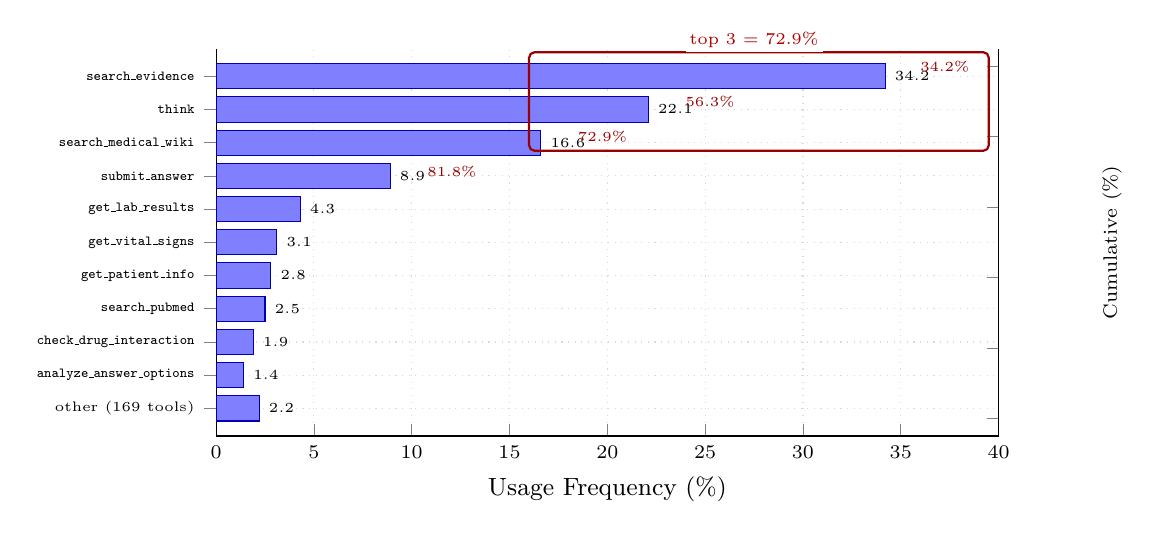
\begin{tikzpicture}
\begin{axis}[
    width=0.95\columnwidth,
    height=6.5cm,
    xbar,
    bar width=0.32cm,
    xlabel={Usage Frequency (\%)},
    xmin=0, xmax=40,
    ytick=data,
    yticklabels={
        other (169 tools),
        \texttt{analyze\_answer\_options},
        \texttt{check\_drug\_interaction},
        \texttt{search\_pubmed},
        \texttt{get\_patient\_info},
        \texttt{get\_vital\_signs},
        \texttt{get\_lab\_results},
        \texttt{submit\_answer},
        \texttt{search\_medical\_wiki},
        \texttt{think},
        \texttt{search\_evidence}
    },
    yticklabel style={font=\fontsize{5.5}{6.5}\selectfont},
    tick label style={font=\scriptsize},
    label style={font=\small},
    grid=major,
    grid style={dotted, gray!30},
    nodes near coords,
    every node near coord/.append style={font=\fontsize{5.5}{6.5}\selectfont, anchor=west},
    axis y line*=left,
    axis x line*=bottom,
    enlarge y limits={abs=0.35cm},
]
\addplot[fill=blue!50!white, draw=blue!70!black] coordinates {
    (2.2, 0)
    (1.4, 1)
    (1.9, 2)
    (2.5, 3)
    (2.8, 4)
    (3.1, 5)
    (4.3, 6)
    (8.9, 7)
    (16.6, 8)
    (22.1, 9)
    (34.2, 10)
};
\end{axis}

% Pareto cumulative overlay
\begin{axis}[
    width=0.95\columnwidth,
    height=6.5cm,
    xmin=0, xmax=40,
    ymin=-0.5, ymax=10.5,
    axis y line*=right,
    axis x line=none,
    ylabel={Cumulative (\%)},
    ylabel style={font=\scriptsize, at={(1.12,0.5)}},
    ytick={0,2,4,6,8,10},
    yticklabels={},
    tick label style={font=\scriptsize},
    clip=false,
]
% Cumulative line (plotted at each bar's y-position, x = cumulative %)
% Cumulative from top: 34.2, 56.3, 72.9, 81.8, 86.1, 89.2, 92.0, 94.8, 96.7, 98.6, 100
% We'll overlay a secondary x-axis concept via normalized positions
% Instead, annotate key cumulative points
\node[font=\fontsize{5.5}{6.5}\selectfont, red!60!black, anchor=west] at (axis cs:35.5, 10) {34.2\%};
\node[font=\fontsize{5.5}{6.5}\selectfont, red!60!black, anchor=west] at (axis cs:23.5, 9) {56.3\%};
\node[font=\fontsize{5.5}{6.5}\selectfont, red!60!black, anchor=west] at (axis cs:18.0, 8) {72.9\%};
\node[font=\fontsize{5.5}{6.5}\selectfont, red!60!black, anchor=west] at (axis cs:10.3, 7) {81.8\%};

% Annotation box for top 3
\draw[red!60!black, thick, rounded corners=2pt] (axis cs:16.0, 7.6) rectangle (axis cs:39.5, 10.4);
\node[font=\fontsize{6}{7}\selectfont, red!70!black, anchor=south, fill=white, inner sep=1.5pt] at (axis cs:27.5, 10.4) {top 3 = 72.9\%};

\end{axis}
\end{tikzpicture}
\caption{Tool usage distribution during TT-OPD training (v16, aggregated over 60 steps). The top 3 tools (\texttt{search\_evidence}, \texttt{think}, \texttt{search\_medical\_wiki}) account for 72.9\% of all tool invocations, reflecting the agent's evidence-gathering strategy. The long tail of 169 domain-specific tools collectively accounts for only 2.2\%, indicating highly selective tool use.}
\label{fig:tool_usage}
\end{figure}


% ============================================================
% Figure 8: Multi-Turn Trajectory Example
% ============================================================
\begin{figure*}[t]
\centering
\resizebox{0.95\textwidth}{!}{%
\begin{tikzpicture}[
    node distance=0.3cm,
    sysbox/.style={rectangle, draw=gray!50, fill=gray!5, rounded corners=3pt, text width=5.5cm, minimum height=0.8cm, align=left, font=\scriptsize, line width=0.5pt},
    stubox/.style={rectangle, draw=blue!55, fill=blue!6, rounded corners=3pt, text width=5.5cm, minimum height=0.8cm, align=left, font=\scriptsize, line width=0.6pt},
    toolbox/.style={rectangle, draw=teal!55, fill=teal!5, rounded corners=3pt, text width=5.5cm, minimum height=0.6cm, align=left, font=\scriptsize, line width=0.5pt},
    tchbox/.style={rectangle, draw=green!60!black, fill=green!5, rounded corners=3pt, text width=5.5cm, minimum height=0.8cm, align=left, font=\scriptsize, line width=0.6pt},
    hintbox/.style={rectangle, draw=orange!70, fill=orange!8, rounded corners=3pt, text width=5.5cm, minimum height=0.6cm, align=left, font=\scriptsize, line width=0.6pt},
    klbox/.style={rectangle, draw=purple!55, fill=purple!5, rounded corners=3pt, text width=2.0cm, minimum height=0.5cm, align=center, font=\scriptsize, line width=0.5pt},
    turnlbl/.style={font=\scriptsize\bfseries, color=gray!60!black},
    privstar/.style={star, star points=5, draw=orange!70, fill=orange!25, minimum size=0.3cm, inner sep=0pt, line width=0.5pt},
    arr/.style={->, >=stealth, thick, gray!50},
    divider/.style={dashed, gray!30, line width=0.5pt},
]

% ====== LEFT COLUMN: Student trajectory ======
\node[turnlbl] (t1lbl) at (0, 0) {Turn 1};

\node[stubox, below=0.15cm of t1lbl, anchor=north] (s1) {
    \textcolor{blue!60!black}{\textbf{Student} $\theta_S$:} \textit{``Let me analyze the patient's symptoms. The presentation of acute chest pain with diaphoresis and ST elevation in leads II, III, aVF suggests inferior STEMI. I need to gather more evidence.''}
};

\node[toolbox, below=0.15cm of s1] (tool1) {
    \textcolor{teal!60!black}{\texttt{search\_evidence}(\text{``inferior STEMI management acute''})}\\[2pt]
    \textcolor{gray!60}{$\rightarrow$ 3 passages retrieved (ACC/AHA STEMI guidelines...)}
};

% Turn 2
\node[turnlbl, below=0.5cm of tool1] (t2lbl) {Turn 2};

\node[stubox, below=0.15cm of t2lbl, anchor=north] (s2) {
    \textcolor{blue!60!black}{\textbf{Student} $\theta_S$:} \textit{``Based on the evidence, the patient has inferior STEMI. The recommended treatment is immediate PCI within 90 minutes. I will submit my answer.''}
};

\node[toolbox, below=0.15cm of s2] (tool2) {
    \textcolor{teal!60!black}{\texttt{submit\_answer}(\text{``Inferior STEMI --- emergent PCI''})}\\[2pt]
    \textcolor{red!60!black}{\ding{55} \textbf{Incorrect}} --- missed right ventricular involvement
};

% Turn 3 label
\node[turnlbl, below=0.5cm of tool2] (t3lbl) {Turn 3 (with TT-OPD)};

% ====== DIVIDER ======
\draw[divider] (-3.2, -6.8) -- (9.5, -6.8);
\node[font=\scriptsize\itshape, color=gray!50, fill=white, inner sep=2pt] at (3.0, -6.8) {Outcome-privileged teacher conditioning};

% ====== RIGHT-SHIFTED: Teacher version ======

% Hint injection
\node[hintbox, below=0.4cm of t3lbl, anchor=north] (hint) {
    \node[privstar] at (-0.15, 0) {};
    \textcolor{orange!70!black}{\textbf{Privileged Hint} (teacher only):}\\
    \textit{``Some aspects of the diagnosis need re-examination. Consider whether additional findings (e.g., right-sided leads, hemodynamic assessment) might change the treatment approach.''}
};

% Teacher response
\node[tchbox, below=0.2cm of hint] (tch) {
    \textcolor{green!50!black}{\textbf{Teacher} $\theta_T$ (with hint):} \textit{``The inferior STEMI diagnosis is partially correct, but ST elevation in V4R should prompt evaluation for RV infarction, which contraindicates nitroglycerin and aggressive fluid resuscitation. The management plan requires modification.''}
};

% KL target boxes on the right
\node[klbox, right=0.8cm of s1.east, anchor=west] (kl1) {
    $D_{\text{KL}}^{(t=1)}$\\[1pt]
    \textcolor{purple!60}{0.012}
};
\draw[arr, purple!40] (s1.east) -- (kl1.west);

\node[klbox, right=0.8cm of s2.east, anchor=west] (kl2) {
    $D_{\text{KL}}^{(t=2)}$\\[1pt]
    \textcolor{purple!60}{0.089}
};
\draw[arr, purple!40] (s2.east) -- (kl2.west);

\node[klbox, right=0.8cm of tch.east, anchor=west] (kl3) {
    $D_{\text{KL}}^{(t=3)}$\\[1pt]
    \textcolor{purple!60}{0.341}
};
\draw[arr, purple!40] (tch.east) -- (kl3.west);

% Arrow showing KL increases with incorrectness
\draw[->, >=stealth, purple!50, thick] ([xshift=0.1cm]kl1.south) -- ([xshift=0.1cm]kl2.north);
\draw[->, >=stealth, purple!50, thick] ([xshift=0.1cm]kl2.south) -- ++(0, -2.3) -- ([xshift=0.1cm]kl3.north);
\node[font=\fontsize{5}{6}\selectfont, purple!50!black, rotate=-90, anchor=south] at ([xshift=0.7cm]kl2.east) {KL increases $\rightarrow$ stronger correction};

% Legend
\node[draw=gray!40, fill=white, rounded corners=3pt, font=\fontsize{5.5}{6.5}\selectfont, align=left, anchor=north west, inner sep=4pt] at (-3.0, -9.5) {
    \textcolor{blue!60!black}{$\blacksquare$} Student trajectory \quad
    \textcolor{teal!60!black}{$\blacksquare$} Tool call/response \quad
    \textcolor{orange!70!black}{$\bigstar$} Privileged hint (teacher only) \quad
    \textcolor{green!50!black}{$\blacksquare$} Teacher (outcome-aware) \quad
    \textcolor{purple!60}{$\blacksquare$} Turn-level KL
};

\end{tikzpicture}%
}%
\caption{Multi-turn trajectory example illustrating TT-OPD. The student generates a 2-turn trajectory (search evidence $\rightarrow$ submit answer), producing an incorrect diagnosis that misses right ventricular involvement. The teacher receives an outcome-privileged hint (\textcolor{orange!70!black}{$\bigstar$}, visible only during teacher logprob computation) and generates an outcome-aware response. Turn-level KL divergence increases from 0.012 (Turn 1, reasonable reasoning) to 0.341 (Turn 3, corrective signal), providing dense per-turn supervision that is strongest where the student most needs correction.}
\label{fig:trajectory_example}
\end{figure*}
